\documentclass{ctexart}
\usepackage{graphicx}
\usepackage{caption}
\usepackage{float}
\usepackage{amsmath}
\usepackage{fancyhdr}
\usepackage{xunicode-addon}
\usepackage{booktabs}
\usepackage{listings}
\usepackage{hyperref}
\usepackage{longtable}
\usepackage[a4paper,hmargin=1.25in,vmargin=1in]{geometry}
% !TeX program = xelatex
\lstdefinestyle{mystyle}{
  basicstyle=\ttfamily\footnotesize,
  breakatwhitespace=false,         
  breaklines=true,                 
  captionpos=b,                    
  keepspaces=true,                 
  numbers=left,                    
  numbersep=5pt,                  
  showspaces=false,                
  showstringspaces=false,
  showtabs=false,                  
  tabsize=2
}

\lstset{style=mystyle}

\title{\begin{figure}[H]
	\centering 
	\includegraphics[height=7cm,width=14cm]{E:/Pictures/中科大.jpg}
	\end{figure}\Huge\textbf{图书馆管理系统课程设计报告}}
\date{}
\punctstyle{banjiao} 
\pagestyle{fancy}
	\fancyhead[C]{\LARGE\textbf{图书馆管理系统}}
	\fancyhead[L]{}
	\fancyhead[R]{}
	\fancyfoot[C]{\thepage}
\begin{document}
	\maketitle
	\thispagestyle{empty}
	
	\[\makebox{\Large{姓名:\underline{\makebox[5cm]{高茂航、李宇湘}}}}\]
	
	$$\makebox{\Large{日期:\underline{\makebox[5cm]{2024.7.20}}}}$$
	
	\clearpage

	\pagenumbering{arabic}

	\section{}
	
	
	
	\section{}

	
	
	\section{数据库概念结构设计}
	\begin{figure}[H]
		\centering 
		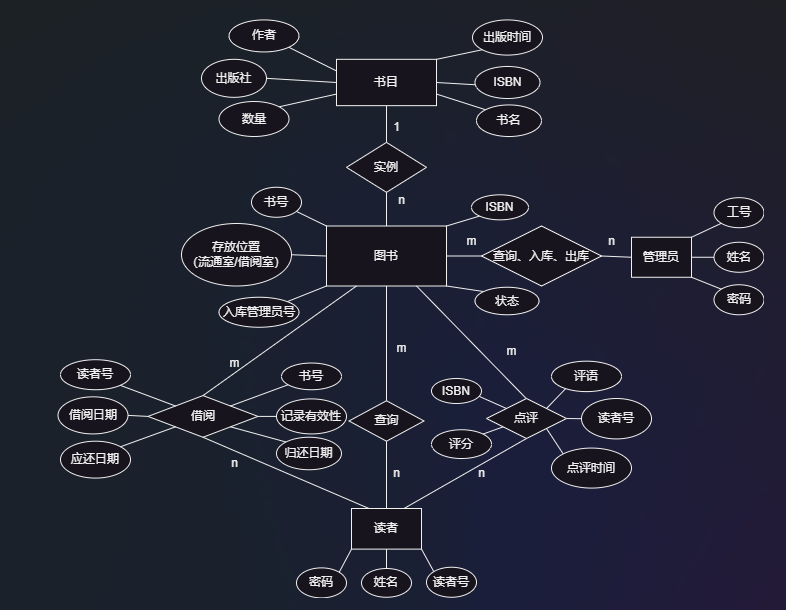
\includegraphics[height=10cm,width=12cm]{ER.png}
		\caption{ER图}
	\end{figure}

	\section{数据库逻辑结构设计}
	\subsection{数据库表结构}
	\begin{longtable}{p{3.5cm}p{3.5cm}p{5.5cm}}
		\toprule
		\textbf{表名 (表名含义)} & \textbf{列名 (注释)} & \textbf{数据类型} \\
		\midrule
		\endhead
		dzTable (读者表) & \underline{dzid} (读者ID) & AutoField \\
		& psw (密码) & CharField(max\_length=256) \\
		& xm (姓名) & CharField(max\_length=10) \\
		\midrule
		tsglyTable (图书管理员表) & \underline{glyid} (管理员ID) & CharField(max\_length=10) \\
		& psw (密码) & CharField(max\_length=256) \\
		& xm (姓名) & CharField(max\_length=10) \\
		\midrule
		smTable (书目表) & \underline{isbn} & CharField(max\_length=50) \\
		& sm (书名) & CharField(max\_length=50) \\
		& zz (作者) & CharField(max\_length=50) \\
		& cbs (出版社) & CharField(max\_length=50) \\
		& cbny (出版时间) & DateTimeField \\
		& count (数量) & IntegerField(default=0) \\
		\midrule
		tsTable (图书实例表) & \underline{tsid} (图书ID) & AutoField \\
		& isbn (对应书目) & ForeignKey(smTable) \\
		& cfwz (存放位置) & CharField(max\_length=20) \\
		& zt (状态) & CharField(max\_length=20) \\
		& jbr (入库该书管理员工号) & ForeignKey(tsglyTable) \\
		\midrule
		BookReview (书评表) & \underline{dzid} (读者ID) & ForeignKey(dzTable) \\
		& \underline{isbn}& ForeignKey(smTable) \\
		& score (评分) & IntegerField(validators=[0,10]) \\
		& comment (评论) & TextField(max\_length=300, null=True) \\
		& comment\_time (评论时间) & DateTimeField(auto\_now\_add=True) \\
		\midrule
		jsTable (借书表) & \underline{dzid} (读者ID) & ForeignKey(dzTable) \\
		& \underline{tsid} (图书ID) & ForeignKey(tsTable, null=True) \\
		& \underline{jysj} (借阅时间) & DateTimeField \\
		& yhsj (应还时间) & DateTimeField \\
		& ghsj (归还时间) & DateTimeField(null=True) \\
		& is\_valid (记录是否有效) & BooleanField(default=True) \\
		\bottomrule
		\end{longtable}
		\subsection{具体分析}

		\subsubsection{dzTable (读者表)}
\begin{itemize}
    \item \textbf{结构}: 包含读者ID(主键)、密码、姓名。
    \item \textbf{解释}: 此表用于存储图书馆读者的基本信息。
    \item \textbf{3NF分析}: 满足3NF,因为每个非主属性完全函数依赖于主键(读者ID),不存在传递依赖或部分依赖。
    \item \textbf{BCNF分析}: 满足BCNF,由于不存在非主属性对主键的部分或传递依赖,同时每个候选键也是超键。
    \item \textbf{4NF分析}: 满足4NF,因为表中不存在多值依赖。
\end{itemize}

\subsubsection{tsglyTable (图书管理员表)}
\begin{itemize}
    \item \textbf{结构}: 包含管理员ID(主键)、密码、姓名。
    \item \textbf{解释}: 此表用于存储图书管理员的基本信息。
    \item \textbf{3NF分析}: 满足3NF,每个非主属性完全函数依赖于主键(管理员ID),不存在传递依赖或部分依赖。
    \item \textbf{BCNF分析}: 满足BCNF,因为不存在非主属性对主键的部分或传递依赖,且每个候选键也是超键。
    \item \textbf{4NF分析}: 满足4NF,因为表中不存在多值依赖。
\end{itemize}

\subsubsection{smTable (书目表)}
\begin{itemize}
    \item \textbf{结构}: 包含国际标准书号ISBN(主键)、书名、作者、出版社、出版时间、数量。
    \item \textbf{解释}: 此表记录了图书的详细信息。
    \item \textbf{3NF分析}: 满足3NF,因为每个非主属性完全函数依赖于主键(ISBN),不存在传递依赖或部分依赖。
    \item \textbf{BCNF分析}: 满足BCNF,因为不存在非主属性对主键的部分或传递依赖,且每个候选键也是超键。
    \item \textbf{4NF分析}: 满足4NF,因为表中不存在多值依赖。
\end{itemize}

\subsubsection{tsTable (图书实例表)}
\begin{itemize}
    \item \textbf{结构}: 包含图书ID(主键)、对应书目的ISBN、存放位置、状态、经办人。
    \item \textbf{解释}: 此表记录了图书馆中每本图书的具体实例信息。
    \item \textbf{3NF分析}: 满足3NF,因为每个非主属性完全函数依赖于主键(图书ID),不存在传递依赖或部分依赖。
    \item \textbf{BCNF分析}: 满足BCNF,因为不存在非主属性对主键的部分或传递依赖,且每个候选键也是超键。
    \item \textbf{4NF分析}: 满足4NF,因为表中不存在多值依赖。
\end{itemize}

\subsubsection{BookReview (书评表)}
\begin{itemize}
    \item \textbf{结构}: 包含读者ID、ISBN、评分、评论、评论时间,其中读者ID和ISBN共同构成复合主键。
    \item \textbf{解释}: 此表用于存储读者对图书的评分和评论。
    \item \textbf{3NF分析}: 满足3NF,因为每个非主属性完全函数依赖于复合主键(读者ID和ISBN),不存在传递依赖或部分依赖。
    \item \textbf{BCNF分析}: 满足BCNF,因为不存在非主属性对复合主键的部分或传递依赖,且每个候选键也是超键。
    \item \textbf{4NF分析}: 满足4NF,因为表中不存在多值依赖。
\end{itemize}

\subsubsection{jsTable (借书表)}
\begin{itemize}
    \item \textbf{结构}: 包含读者ID、图书ID、借阅时间、应还时间、归还时间、记录是否有效,其中读者ID、图书ID和借阅时间共同构成复合主键。
    \item \textbf{解释}: 此表记录了读者借阅图书的详细信息。
    \item \textbf{3NF分析}: 满足3NF,因为每个非主属性完全函数依赖于复合主键(读者ID、图书ID和借阅时间),不存在传递依赖或部分依赖。
    \item \textbf{BCNF分析}: 满足BCNF,因为不存在非主属性对复合主键的部分或传递依赖,且每个候选键也是超键。
    \item \textbf{4NF分析}: 满足4NF,因为表中不存在多值依赖。
\end{itemize}

\subsection{总结}
所有表均满足第三范式(3NF)和BCNF的要求,
因为它们的每个非主属性都直接依赖于主键(或复合主键),
并且不存在任何传递依赖或部分依赖。此外,所有表也满足第四范式(4NF),
因为它们的表结构比较简单,不存在多值依赖。这样的设计确保了数据的一致性、减少了数据冗余,并且提高了查询效率。
	\section{}
	\section{}

	

\end{document}